\section{FlexGen}
\begin{frame}{FlexGen: Goal}

\begin{itemize}
\item LLMs is too large to fit into the memory of a single GPU, design efficient \underline{\hl{offloading strategies}} for \underline{\textcolor{blue}{high-throughput}} (sacrifice latency) generative inference on \underline{\hl{a single commodity GPU}}.
\item Run an LLM with limited GPU memory, offload it to secondary storage and perform computation part-by-part by partially loading it.
\end{itemize}
\begin{figure}
    \centering
    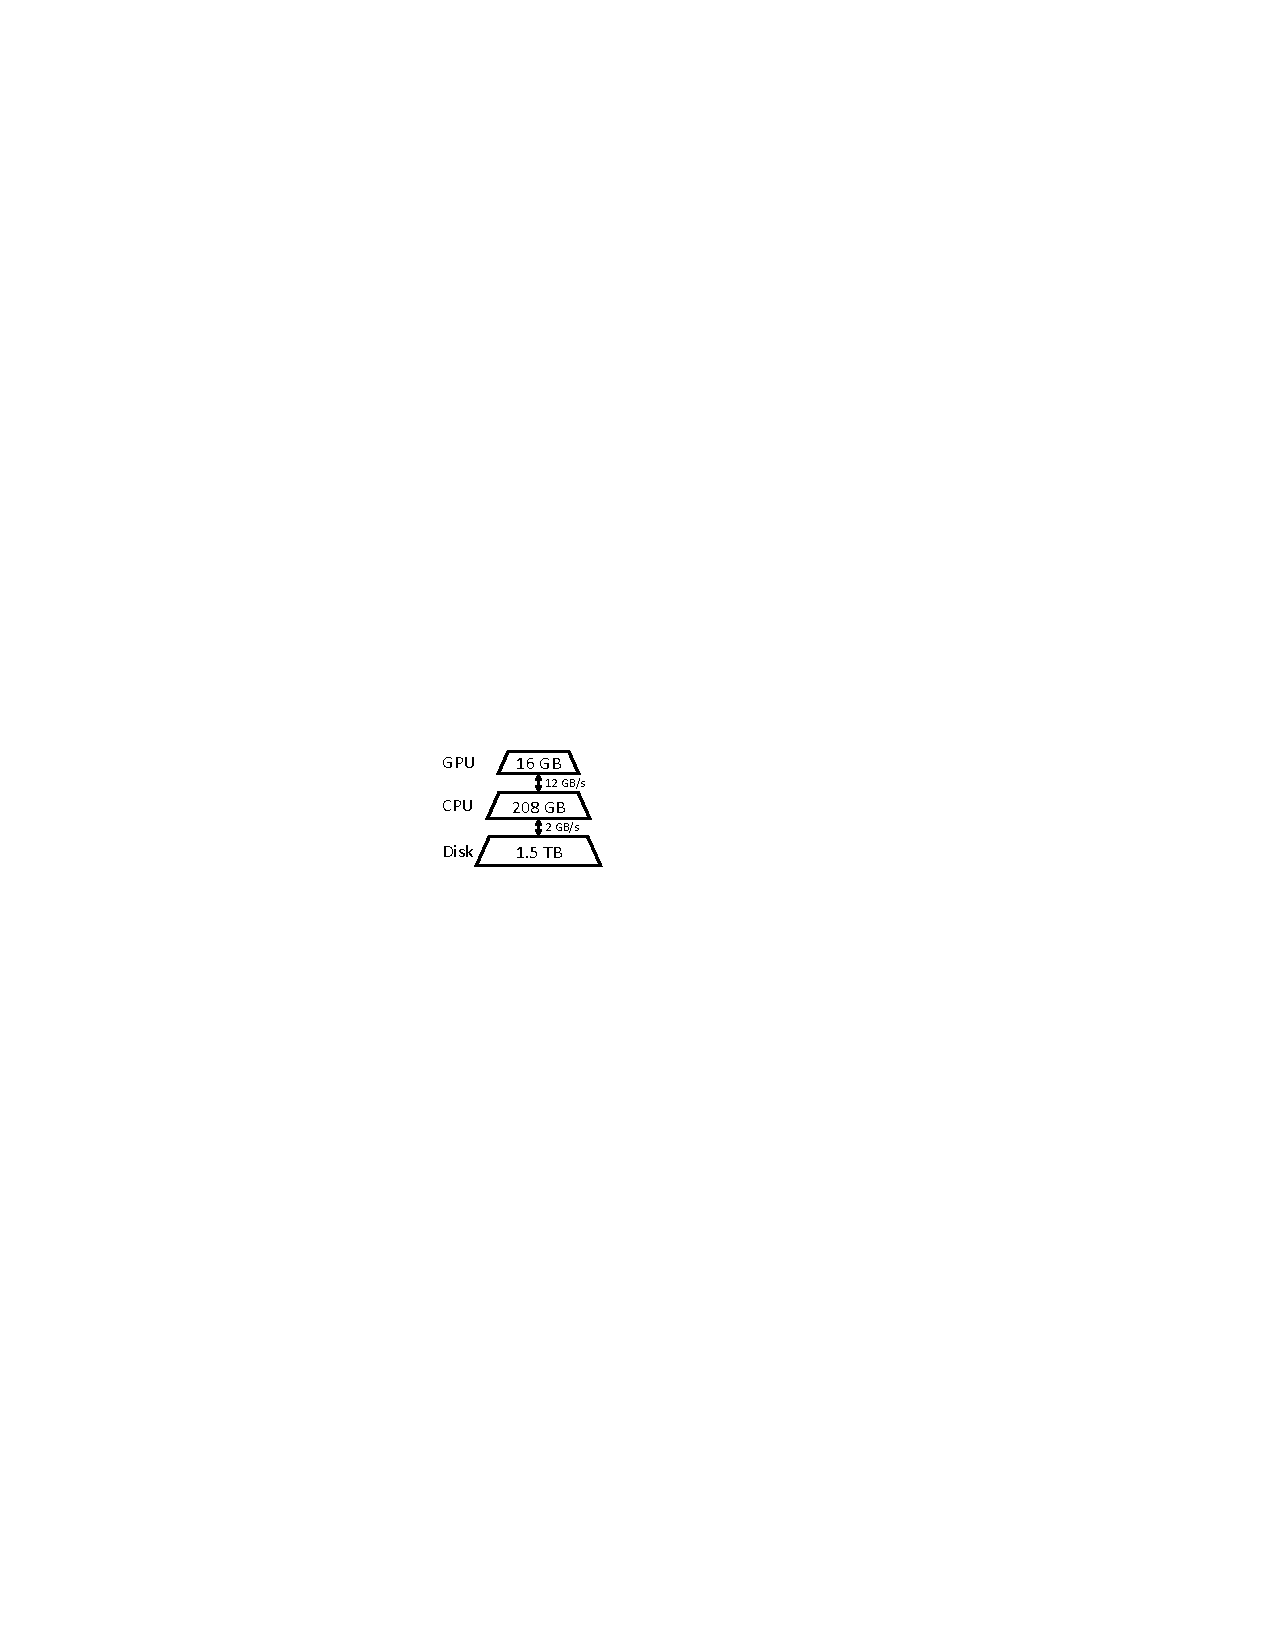
\includegraphics[width=.3\textwidth]{./images/memory-system.pdf}
\end{figure}

\end{frame}

\begin{frame}{FlexGen: Problem Formulation}
\begin{figure}
    \centering{
    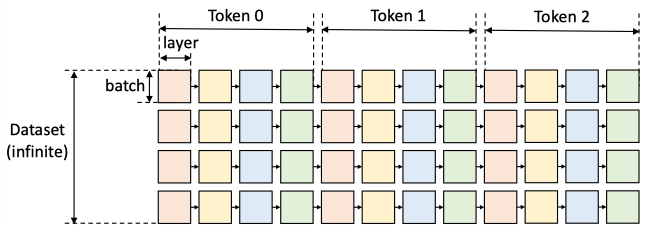
\includegraphics[width=0.6\linewidth]{./images/LLM-inference-graph.png}
    \caption{Computational graph of LLM inference.}
    }
\end{figure}

\footnotesize{

The generative inference with offloading is \hl{a graph traversal problem}. Figure out a valid path that traverses all squares, while \hl{subject to the constraints}:

\begin{enumerate}
    \item A square can only be computed if all squares to its left on the same row were computed.
    \item To compute a square on a device, all its inputs must be loaded to the same device.
    \item The activations should be stored until its right sibling is computed. \item The KV cache should be stored until the rightmost square on the same.
    \item At any time, the total size of tensors stored on a device cannot exceed its memory capacity.
\end{enumerate}
}
\end{frame}

\begin{frame}{Block Schedule: Throughput vs. Latency}
    \begin{columns}[c]
        \begin{column}{.5\textwidth}
        \begin{figure}
            \centering
            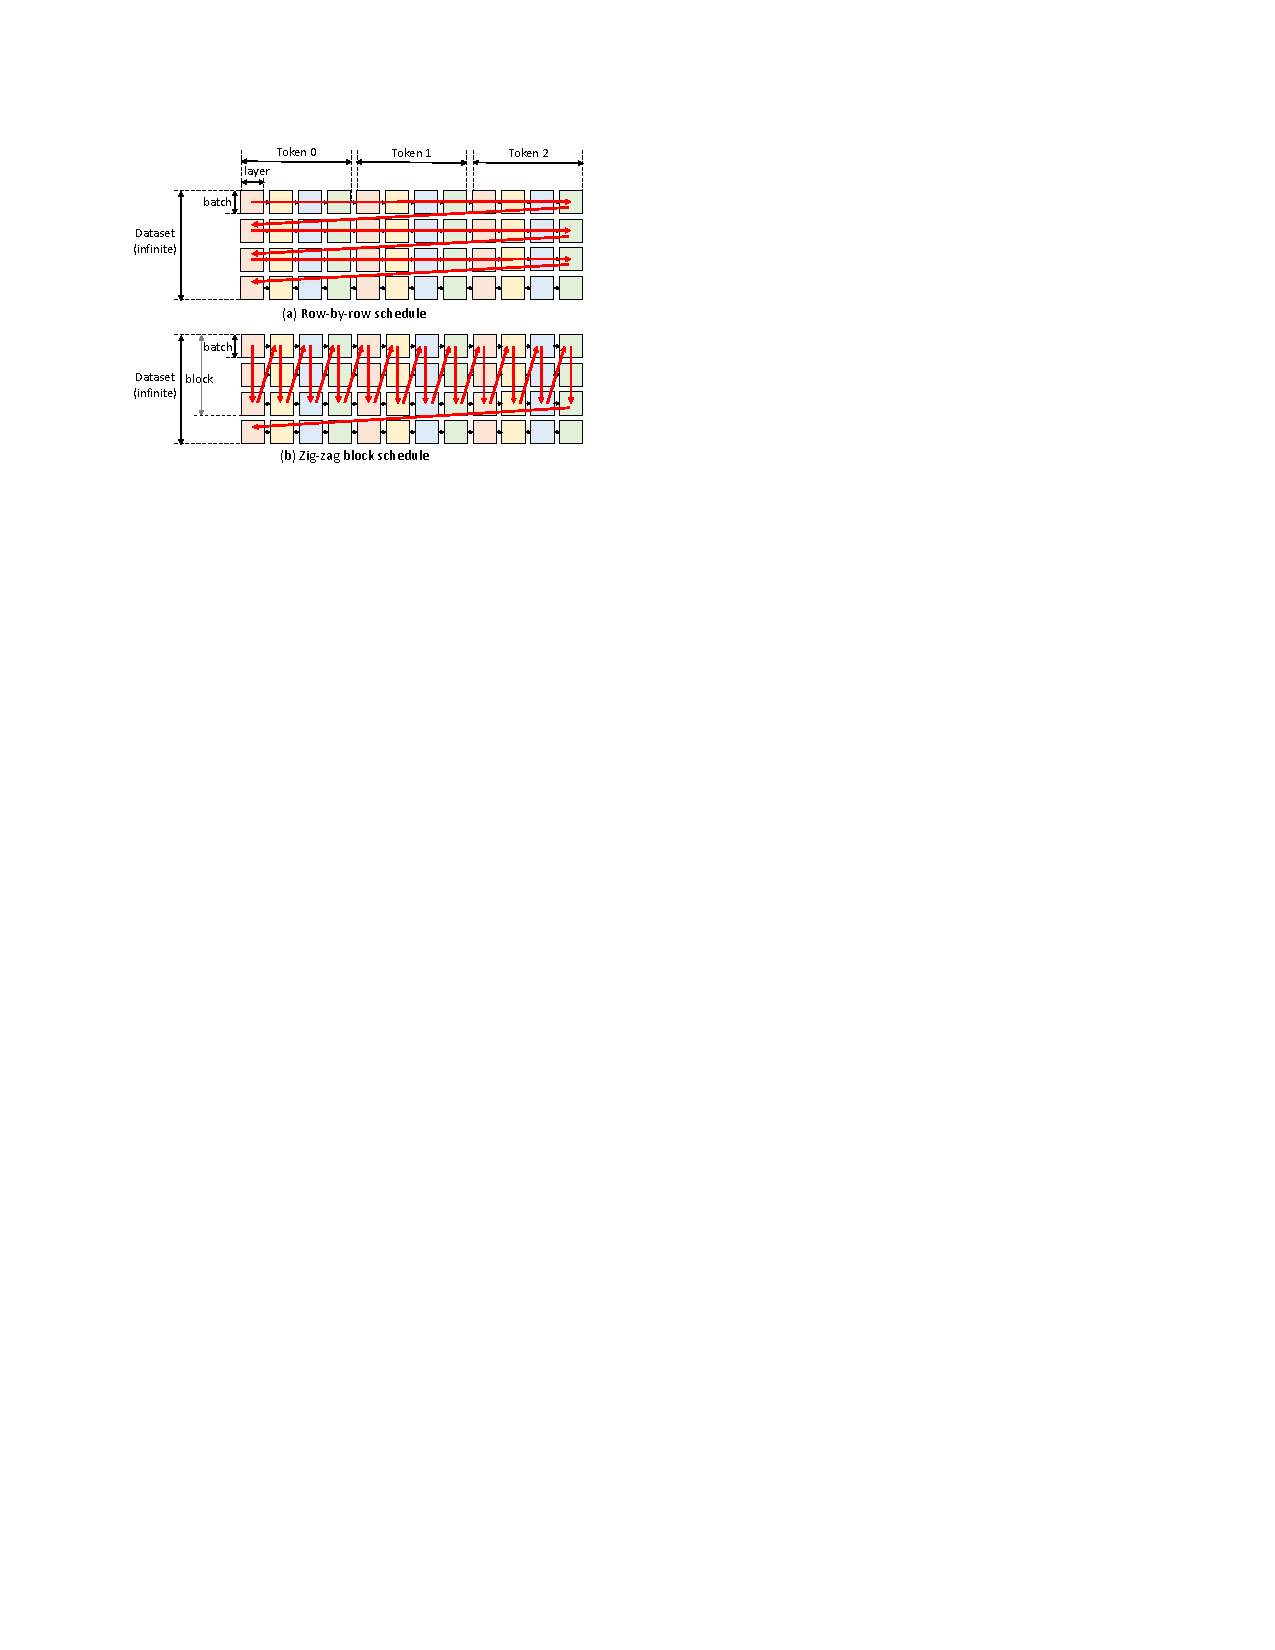
\includegraphics[width=1.\textwidth]{./images/block-schedule.pdf}
            \caption{Virtualizing the block scheduling.}
        \end{figure}      
        \end{column}
    
        \begin{column}{.5\textwidth}
            \begin{figure}
                \centering
                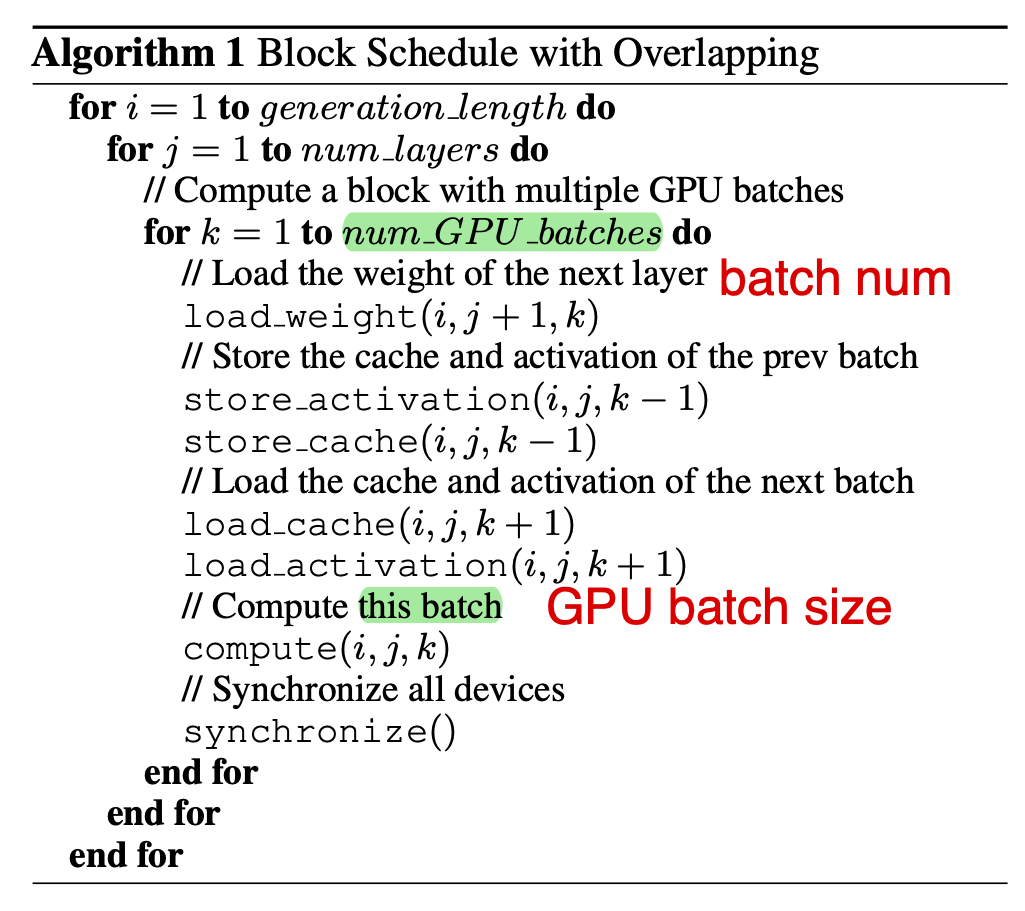
\includegraphics[width=1.\textwidth]{./images/block-schedule-algorithm.png}
                \caption{The block scheduling algorithm.}
            \end{figure}  
        \end{column}
    \end{columns}  
\end{frame}

\begin{frame}{The Search Space}
    \begin{enumerate}
        \footnotesize{
        \item \textbf{Block scheduling algorithm} searches two hyper parameters: batch size and batch nummbers.
        \item \textbf{Tensor placement} searches how to store weights, activations, K-V caches on device.
        \begin{itemize}
            \scriptsize{
            \item $wg$, $wc$, $wd$ define the percentages of weights stored on GPU, CPU, and disk
            \item  $hg$, $hc$, $hd$ define the percentages of activations stored on GPU, CPU, and disk
            \item $cg$, $cc$, $cd$ define the percentages of k-V cache stored on GPU, CPU, and disk
            }
        \end{itemize}
        }
        \item \textbf{Computation delegation}: using CPU compute can still be beneficial in some cases.
        \begin{itemize}
            \scriptsize{
            \item The size of move $KV$ cache is $b \times s \times d \times 4$;
            \item The size of move activation is $b \times d$;
            \item Compute attention scores on CPU reduce I/O by $s\times$, if the accociated $KV$ cache is not stored on GPU, compute attention scores on CPU would be better.
            }
        \end{itemize}
    \end{enumerate}
\end{frame}

\begin{frame}{Cost Model and Policy Search}

    \small{\textbf{Cost model: a mixture of latency and peak memory usage prediction}}

    \begin{itemize}
        \footnotesize{
        \item Latency prediction
        \begin{enumerate}
            \footnotesize{
            \item \textcolor{red}{I/O term} is estimated by summing by all the I/O events, \textcolor{blue}{computation term} is estimated by summing up all computation events. Assume perfect overlapping}
        \end{enumerate}
        \begin{align*}
            T &= T_{pre}\cdot l+ T_{gen} \cdot (n-1) \cdot l \\
            T_{pre} &= \max(\textcolor{red}{ctog^p}, \textcolor{red}{gtoc^p}, \textcolor{red}{dtoc^p}, \textcolor{red}{ctod^p}, \textcolor{blue}{comp^p}) \\
            T_{gen} &= \max(\textcolor{red}{ctog^g}, \textcolor{red}{gtoc^g},\textcolor{red}{dtoc^g},\textcolor{red}{ctod^g}, \textcolor{blue}{comp^g})
        \end{align*}
        }
        \item The ILP to solve 11 variable:
        \begin{figure}
            \centering
            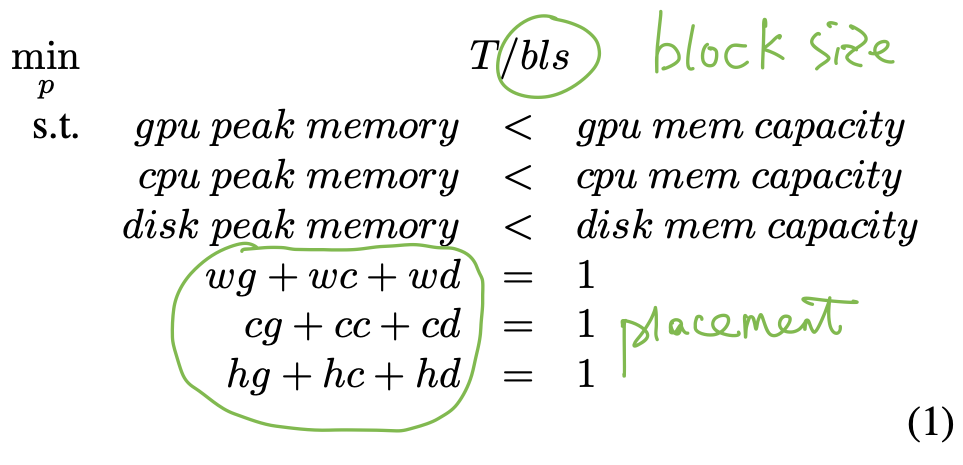
\includegraphics[width=.5\textwidth]{./images/ILP.png}
            \caption{The ILP problem.}
        \end{figure}  
    \end{itemize}
\end{frame}